\documentclass{article}
\usepackage{float}
\usepackage[T2A]{fontenc}
\usepackage[utf8]{inputenc}
%\usepackage[cp1251]{inputenc}


\usepackage[russian]{babel}
\usepackage{graphicx}

\begin{document}



\section{Введение}
Тезисы:
\begin{itemize}
\item Выбором структуры модели занимается meta-learning
\item Мы знаем  основные методы порождения моделей, требуется адекватное представление структуры
\item Ссылка на обзоры. В целом, мы не касаемся методов порождения обобщенное-линейных моделей
\item Текст из Степашко:

Если речь идет об анализе методов автоматического порождения аппроксимирующих моделей, то можно описать точный круг решаемых задач и ввести общепризнанные базовые математические объекты, с помощью которых попытаться систематизировать и формализовать то множество способов порождения моделей, которые мы имеем. Педро Домингос мог бы это сделать, например (в Master algorithm), но ограничился популярными высказываниями.

\end{itemize}
\section{Метаоптимизация}
\subsection{Теоретические основания метаобучения }
В работе~\cite{layerwise_optimal} рассматривается задача построения генеративных моделей, предлагается критерий для послойного обучения генеративных моделей:
\begin{figure}[H]
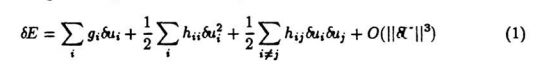
\includegraphics[width=\textwidth]{./arch_review_figs/obd.png}
\end{figure}

В работе~\cite{search_space} рассматриваются подходы к сэмплированию моделей глубокого обучения. Предлагается формализация пространства поиска и формальное описание эл
ементов этого пространства:
 \begin{figure}[H]
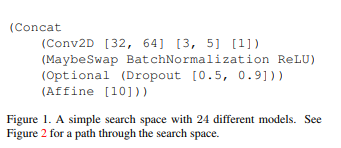
\includegraphics[width=\textwidth]{./arch_review_figs/search_space.png}
\end{figure}

\subsection{Метаоптимизация: learning to learn}
В работе~\cite{self_rnn} предлагается подход к адаптивному изменению структуры сети, основанный на обучении с подкреплением. Предлагается параметризация модели нейросети, включающая в себя модифицирующие и анализирующие выходы, позволяющие модифицировать параметры модели:
\begin{figure}[H]
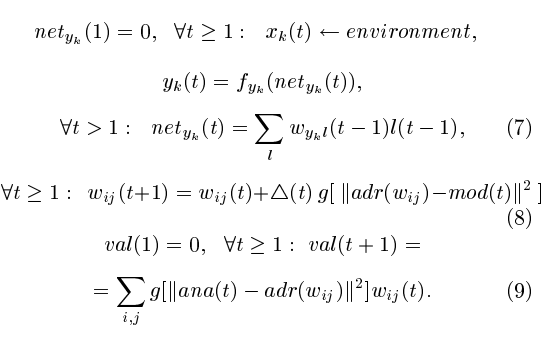
\includegraphics[width=\textwidth]{./arch_review_figs/self_rnn.png}
\end{figure}
Предлагается продолжение подхода, позволяющая рекуррентно продолжать анализ модели и порождать мета-метан-$\dots$-анализ.

В работе~\cite{meta_sgd} рассматривается оптимизация мета-параметров (шага градиентного спуска и начального распределения параметров) с использованием обучения с подкреплением. На каждой итерации сэмплируется подвыборка, по которой проводится оптимизация данных метапараметров:
\begin{figure}[H]
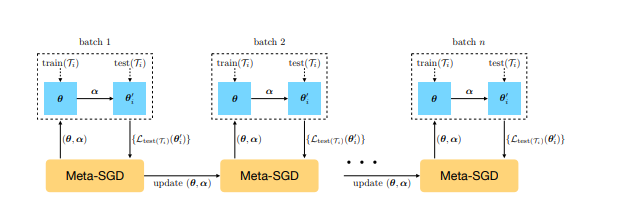
\includegraphics[width=\textwidth]{./arch_review_figs/meta_sgd.png}
\end{figure}

В работе~\cite{l2l} рассматирвается задача восстановления параметров модели по параметрам слабо обученной модели:
\begin{figure}[H]
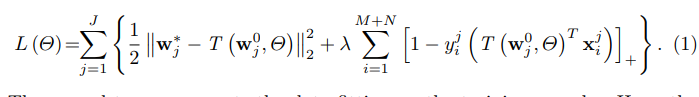
\includegraphics[width=\textwidth]{./arch_review_figs/l2l.png}
\end{figure}

\begin{figure}[H]
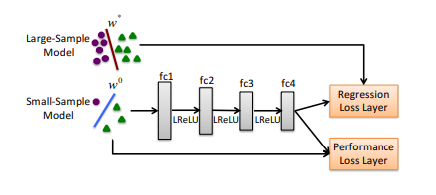
\includegraphics[width=\textwidth]{./arch_review_figs/l2l_scheme.png}
\end{figure}

В работе~\cite{l2l_by_gd_gd} рассматривается оптимизация метапараметров оптимизации с помощью LSTM, которая выступает альтернативе аналитических алгоритмов, таких как Adam или AdaGrad. LSTM имеет  (сравнительно) небольшое количество параметров, т.к. для каждого метапараметра используется своя копия модели LSTM с одинаковыми параметрами для каждой копии:
\begin{figure}[H]
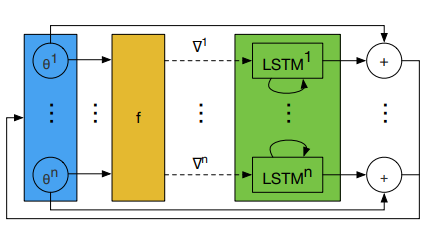
\includegraphics[width=\textwidth]{./arch_review_figs/l2lbygd.png}
\end{figure}






\subsection{Перебор структур}
В работе~\cite{search_smbo} рассматривается задача порождения сверточных нейронных сетей. Предлагается проводить поиск оптимальной структуры сети по восходящему по сложности порядку: начиная от сетей с одни блоком и наращивая блоки. В силу высокой вычислительной сложности данного подхода, вместо построения модели,предлагается обучить рекуррентную нейросеть,которая предсказывает качество модели по заданным блокам. 


В работе~\cite{optimal_racing} рассматривается задача выбора архитектуры с помощью большого количества параллельных запусков обучения моделей, предлагаются критерии ранней остановки оптимизации обучения моделей.


\subsection{ Обучение с подкреплением}
В работе~\cite{reinf} представлена схема выбора архитектуры сверточной нейросети с использованием обучения с подкреплением. В качестве актора (контроллера) выступает рекуррентная нейронная сеть.
\begin{figure}[H]
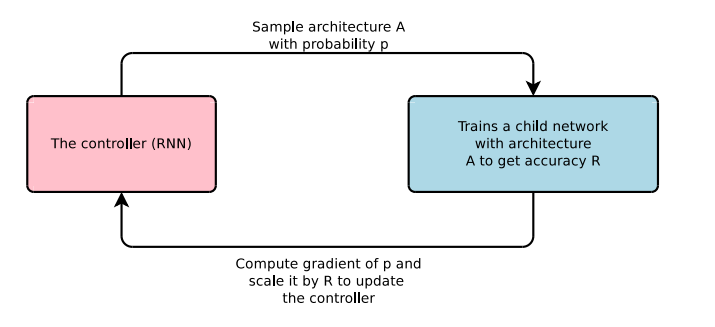
\includegraphics[width=\textwidth]{./arch_review_figs/reinf.png}
\end{figure}
В работе~\cite{reinf_predict} предлагается построение регрессионной модели для оценки финального качества модели и ранней остановки оптимизации моделей. Данный подход позволил существенно ускорить поиск моделей, представленный в работе~\cite{reinf}.
В работе~\cite{reinf_transfer} рассматривается задача переноса архитектуры нейросети, обученной на более простой выборки, на более сложную. Также предлагается параметризация пространства поиска, более делатьное, чем в~\cite{reinf}:
\begin{figure}[H]
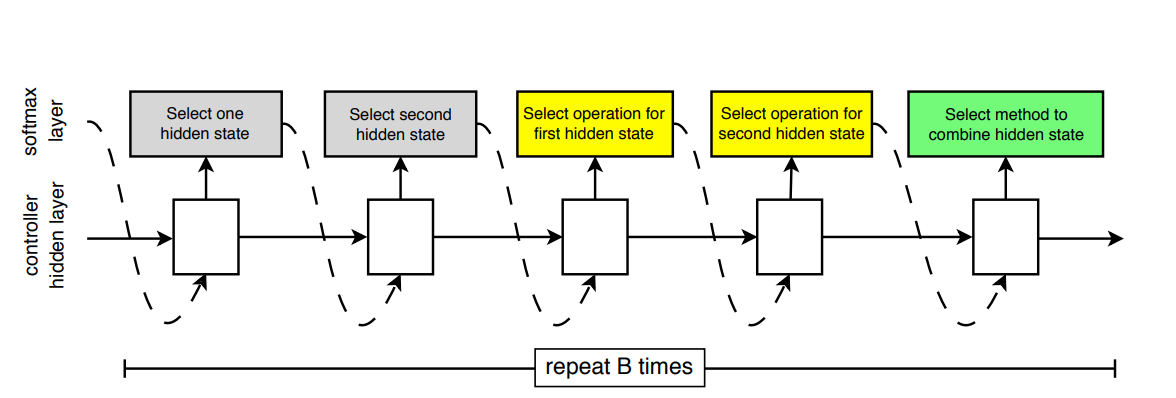
\includegraphics[width=\textwidth]{./arch_review_figs/reinf2.png}
\end{figure}

В отличие от предыдущих работ, в работе~\cite{reinf_deep2net} предлагается подход к инкрементальному обучению нейросети, основанном на модификации модели, полученной на предыдущем шаге. Рассматривается две операции над нейросетью:
\begin{itemize}
\item Расширение сети
\item Углубление сети
\end{itemize}

\begin{figure}[H]
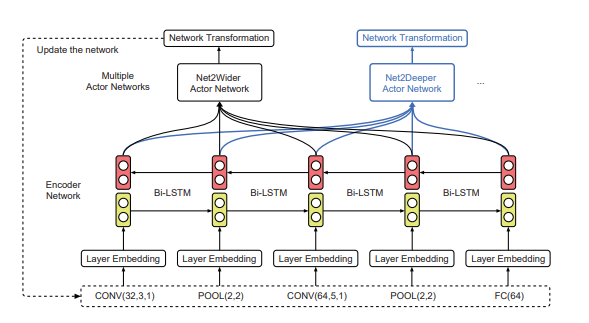
\includegraphics[width=\textwidth]{./arch_review_figs/deep2net.png}
\end{figure}



\section{Адаптивное изменение структуры}
В данном разделе собраны методы изменения структуры существующей модели. 

\paragraph{Алгоритмы наращивания и прореживания параметров модели}
В работе~\cite{obd} предлагается удалять неинформативные параметры модели, где в качестве показателя информативности выступает следующий фнуционал: 
\begin{figure}[H]
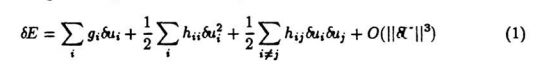
\includegraphics[width=\textwidth]{./arch_review_figs/obd.png}
\end{figure}
В работе~\cite{obs} было предложено развитие данного метода. В данной работе, в отличие от~\cite{obd} не вводится предположений о дигональности Гессиана функции ошибок, поэтому удаление неинформативных параметров модели производится точнее.

В работе~\cite{nips} был предложен метод, основанный на получении вариационной нижней оценки правдоподобия модели. В качестве критерия информативности параметра выступало отношение вероятности нахождения параметра в пределах априорного распределения к вероятности равенста параметра нулю:
\begin{figure}[H]
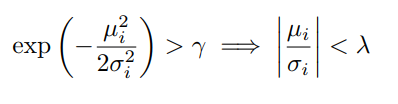
\includegraphics[width=\textwidth]{./arch_review_figs/nips_var.png}
\end{figure}
Идея данного метода была развита в~\cite{bayes_compr}, где также используются вариационные методы. В отличие от предыдущей работы, в данной работе рассматривается ряд априорных распределений параметров, позволяющих прореживать модели более эффективно:
\begin{itemize}
\item Нормальное распределение с лог-равномерным распределением дисперсии, независимой для каждого нейрона:
\begin{figure}[H]
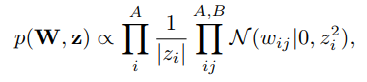
\includegraphics[width=\textwidth]{./arch_review_figs/bayes_compr_group.png}
\end{figure}
\item Произвденеие двух Распределений Half-Cauchy (полу-Коши?): одно ответственно за отдельный параметр, другое --- за общее распределение параметров:
\begin{figure}[H]
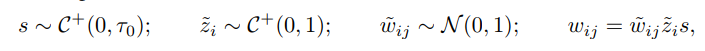
\includegraphics[width=\textwidth]{./arch_review_figs/bayes_compr_cauchy.png}
\end{figure}
\end{itemize}

Смежной темой к прореижванию моделей выступает компрессия нейросетей. Основным отличием задачи прореживания и компрессии выступает эксплуатационное требование: если прореживание используется для получения оптимальной и наиболее устойчивой модели, то компрессия часто производится для сохранения памяти и основных эксплуатационных характеристик исходной модели (?).
В работе~\cite{nvidia_prune}
предлагается итеритавиное использование регуляризации типа DropOut~\cite{dropout} для прореживания модели. 
В работах~\cite{weight_quantization, weight_quantization2} используются методы снижения вычислительной точности представления парамеров модели на основе кластеризации весов.
В работе~\cite{weight_quantization2} предлагается метод компрессии, основанный на кластеризации значений параметров модели и представлении их в сжатом виде на основе кодов Хаффмана.

В работах~\cite{boost_res, adanet} предлагается наращивание моделей, основанное на бустинге. В работе рассматривается задача построения нейросетевых моделей специального типа:
\[
    f_{t+1} = \sigma(f_t) + f_t,
\]
приводится параметризация модели, позволяющая рассматривать декомпозировать модель на слабые классификаторы.
В работе~\cite{adanet} на каждом шаге построения выбирается одно из двух расширений модели, каждое из которых рассматирвается как слабый классификатор:
1. Сделать модель шире
2. Сделать модель глубже
\begin{figure}[H]
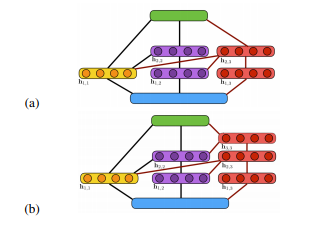
\includegraphics[width=0.5\textwidth]{./arch_review_figs/adanet.png}
\end{figure}
Построение модели заканчивается при условии снижении радемахереовской сложности:
\begin{figure}[H]
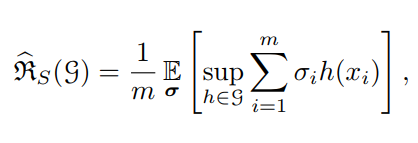
\includegraphics[width=0.5\textwidth]{./arch_review_figs/rad.png}
\end{figure}



\section{Байесовские методы порождения и выбора моделей}
\subsection{Автоматическое определение релевантности параметров}
В работе~\cite{hyper} рассматривается задача оптимизации гиперпараметров.  Авторы предлагают оптимизировать константы $l_2$-регуляризации отдельно для каждого параметра модели, проводится параллель с методами автоматического определения релевантности параметров (ARD)~\cite{MacKay}.

В работе~\cite{ard} рассматривается метод ARD для снижения размерности скрытого пространства вариационных порождающих моделей: скрытая переменная параметризуется как  произведение некоторой случайной величины $\mathbf{z}$  на вектор, отвечающий за релевантность каждой компоненты скрытой переменной:
\begin{figure}[H]
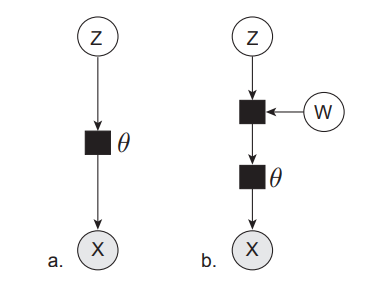
\includegraphics[width=0.5\textwidth]{./arch_review_figs/ard.png}
\end{figure}

\subsection{Суррогаты}
В работе~\cite{bo_gp} предлагается моделировать качество модели гауссовым процессом, параметрами которого выступают гиперпараметры исходной модели.
Модель, аппроксимирующая качество исходной модели, называется суррогатом. 

Одна из основных проблем использования гауссового процесса как суррогатной модели --- кубическая сложность оптимизации. В работе~\cite{random_gaus} предлагается использовать случайные подпространства гиперпараметров для ускоренной оптимизации.  В работе~\cite{gp_tree} предлагается кобминация из множества гауссовых моделей и линейной модели, позволяющая модели нелинейные зависимости гиперпараметров, а также существенно сократить сложность оптимизации. 

В работе~\cite{rbf_surrogate} предлагается рассматривать RBF-модель для аппроксимации качества исходной модели, что позволяет ускорить процесс оптимизации суррогатной модели. В~\cite{snoek_deep} рассматривается глубокая нейронная сеть в качестве суррогатной функции. Вместо интеграла правдоподобия, который оценивается в случае использования гауссового процесса в качестве суррогата, используется максимум апостериорной веротяности.

Важным параметром гауссовых процессов является функиия ядра гауссового процесса, полностью определяющая процесс в случае нулевого среднего. В работе~\cite{gp_fusion} предлагается функция ядра, определенная на графах:
    \[
    k(x,y) = r(d(x,y)),
    \]
где $d$ --- геодезическое расстояние между вершинами графа, $r$ --- некоторая вещественная функция (наверно положительно определенная, но это не указано явно в статье).
В работе~\cite{gp_arc} рассматривается задач выбора структуры нейросети, предлагается ядро специального вида, позволюящее учитывать только те гиперпапараметры, которые есть в обеих сравниваемых моделях: к примеру, для двуслойной и трехслойной нейросети будут уччитываться гиперпараметры, отвечающие только за первые два слоя. 
\begin{figure}[H]
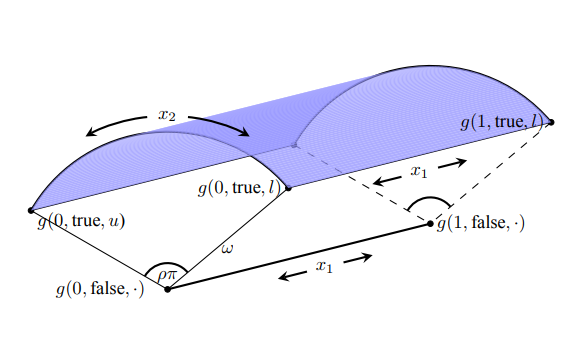
\includegraphics[width=0.5\textwidth]{./arch_review_figs/arc.png}
\end{figure}


\subsection{Адаптивное изменение структуры}

В работе~\cite{cib} рассматривается порождение unsupervised-моделей с использованием расширения процесса Индийского Буфета:
\begin{figure}[H]
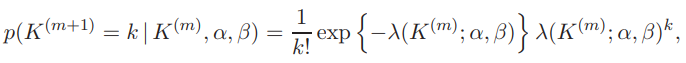
\includegraphics[width=0.5\textwidth]{./arch_review_figs/cib_eq.png}
\end{figure}
\begin{figure}[H]
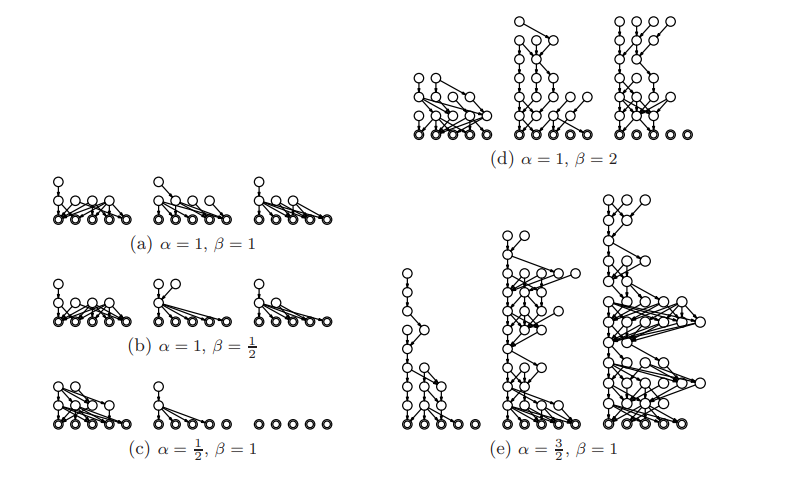
\includegraphics[width=0.5\textwidth]{./arch_review_figs/cib.png}
\end{figure}

В работе~\cite{cib_simple} предлагается упрощенная модель Индийского Буфета:
\begin{figure}[H]
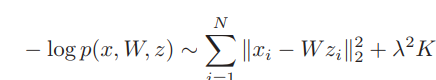
\includegraphics[width=0.5\textwidth]{./arch_review_figs/cib_simple.png}
\end{figure}


Работы по процессу IBP для порождения unsupervised-моделей (иерархических):

%https://www.researchgate.net/profile/Philippe_Giguere/publication/261404006_Learning_the_Structure_of_Probabilistic_Graphical_Models_with_an_Extended_Cascading_Indian_Buffet_Process/links/5532fa4f0cf27acb0deda6ea.pdf

%https://arxiv.org/pdf/1410.4599.pdf
В работе~\cite{shirakawa2018dynamic} предлагается параметризация структуры модели с использованием Бернуллиевских величин:
каждая величина отвечает за включение или выключение слоя сети.



\subsection{Порождающие модели}
https://arxiv.org/pdf/1406.5298.pdf
%Semi-supervised вариационный автокодировщик: добавление Y в порождающую модель


https://arxiv.org/pdf/1603.06277.pdf
TODO, судя по всему - обобщение вариационного кодировщика на произвольные граф модели

https://arxiv.org/pdf/1611.06585.pdf
Предлагается стратегия добавления компонент при вариационном выводе. Проводится аналогия с бустингом.

\subsection{Состязательные модели}
\section{Способы прогнозирования графовых структур}
В разделе собраны ключевые работы по порождению графовых моделей.

\section{Эвристические и прикладные методы}
Прочие работы. 

\bibliographystyle{utf8gost71u}
\bibliography{dis_literature}

\end{document}
